\chapter{Diseño del protocolo de control In-Band}
\label{ch:analisis}

En este capítulo, se abordará una fase fundamental del proyecto, centrada en el diseño de un protocolo de control In-Band para la gestión de redes. En este capítulo, se realizará un exhaustivo análisis de soluciones anteriores basadas en el enfoque In-Band, donde se explorarán diferentes propuestas y se evaluarán sus fortalezas y debilidades.\\
\\
El objetivo principal será definir las funcionalidades básicas que debe poseer el protocolo de control In-Band, considerando los requisitos específicos del proyecto y las necesidades de los entornos de redes actuales. Se examinarán aspectos clave, como la capacidad de establecer una conexión entre los nodos de la red y el controlador, el manejo eficiente del plano de datos para la transmisión de información de control y la escalabilidad para adaptarse a entornos de redes heterogéneas y de gran tamaño. Además, se proporcionará una explicación detallada del funcionamiento del protocolo diseñado, describiendo los diferentes componentes, los mensajes intercambiados entre nodos y controlador, así como los procedimientos de configuración y gestión de la red. Se analizarán las decisiones de diseño tomadas y se justificarán en base a los objetivos del proyecto y las características de los entornos de redes abordados.Por último, se tomará una decisión sobre la plataforma más adecuada para la implementación del protocolo de control In-Band. Se evaluarán diferentes opciones, considerando factores como la disponibilidad de herramientas y tecnologías relevantes, la compatibilidad con los requisitos del proyecto y la viabilidad de su implementación en entornos reales.

%%%%%%%%%%%%%%%%%%%%%%%%%%%%%%%%%%%%%%%%%%%%%%%%%%%%%%%%%%%%%%%%%%%%%%%%%%%%%%%%%%%%%%%%%%%%%%%%%
\section{Protocolo In-Band}
\label{sec:ana_inband}

%%%%%%%%%%%%%%%%%%%%%%%%%%%%%%%%%%%%%%%%%%%%%%%%%%%%%%%%%%%%%%%%%%%%%%%%%%%%%%%%%%%%%%%%%%%%%%%%%
\section{Plataforma de desarrollo y validación}
\label{sec:ana_mininet_wifi}

%%%%%%%%%%%%%%%%%%%%%%%%%%%%%%%%%%%%%%%%%%%%%%%%%%%%%%%%%%%%%%%%%%%%%%%%%%%%%%%%%%%%%%%%%%%%%%%%%
\section{Agente \glsentryshort{sdn}}
\label{sec:ana_switch}

%%%%%%%%%%%%%%%%%%%%%%%%%%%%%%%%%%%%%%%%%%%%%%%%%%%%%%%%%%%%%%%%%%%%%%%%%%%%%%%%%%%%%%%%%%%%%%%%%
\section{Agente de control \glsentryshort{sdn}}
\label{sec:ana_controller}

%%%%%%%%%%%%%%%%%%%%%%%%%%%%%%%%%%%%%%%%%%%%%%%%%%%%%%%%%%%%%%%%%%%%%%%%%%%%%%%%%%%%%%%%%%%%%%%%%
\section{Análisis funcional de la interfaz del \glsentryshort{bofus}}
\label{sec:ana_bofuss}

%%%%%%%%%%%%%%%%%%%%%%%%%%%%%%%%%%%%%%%%%%%%%%%%%%%%%%%%%%%%%%%%%%%%%%%%%%%%%%%%%%%%%%%%%%%%%%%%%
\section{Análisis de la clase \texttt{UserAP} en Mininet-WiFi}
\label{sec:ana_userap}

En esta sección, vamos a sumergirnos en un análisis exhaustivo de la clase \texttt{UserAP} en Mininet-WiFi, una pieza fundamental que envuelve al \gls{bofus}. Al observar detenidamente el diagrama UML de clases en la figura \ref{fig:userAP}, nos encontramos con una intrigante jerarquía de clases relacionadas con \texttt{UserAP}. En el centro de esta estructura se encuentran las clases primigenias, \texttt{Node} y \texttt{Node_wifi}, que se llevan la mayor carga lógica al albergar la mayoría de atributos y métodos esenciales. Estas clases primigenias desempeñan un papel crucial al gestionar una serie de operaciones vitales. Entre sus responsabilidades se encuentran la creación de \textit{Network namespaces}, la configuración y creación de interfaces inalámbricas, el manejo hábil del \gls{tc} para establecer los atributos de los enlaces y mucho más. Son el núcleo de la implementación que permite el funcionamiento armonioso de la infraestructura.\\
\\
No obstante, es importante destacar que la clase \texttt{UserAP}, encargada de encapsular al \gls{bofus}, también aporta su propia lógica especializada. Su tarea principal radica en la gestión del proceso \texttt{HostAPd}, un daemon que trabaja incansablemente para materializar las diversas funcionalidades de punto de acceso. Este componente es fundamental para dotar de vida y dinamismo a la red inalámbrica emulada. Además de su papel esencial en el despliegue del \gls{bofus}, estas clases tienen una responsabilidad adicional: implementar una interfaz de ejecución que permite adaptar las condiciones del escenario a los parámetros necesarios de la interfaz de línea de comandos del software switch \gls{sdn}. Esta adaptabilidad se convierte en una ventaja estratégica, ya que proporciona la flexibilidad necesaria para personalizar y ajustar el entorno según las necesidades específicas de cada caso de uso.
% fig
\begin{figure}[ht]
    \centering
    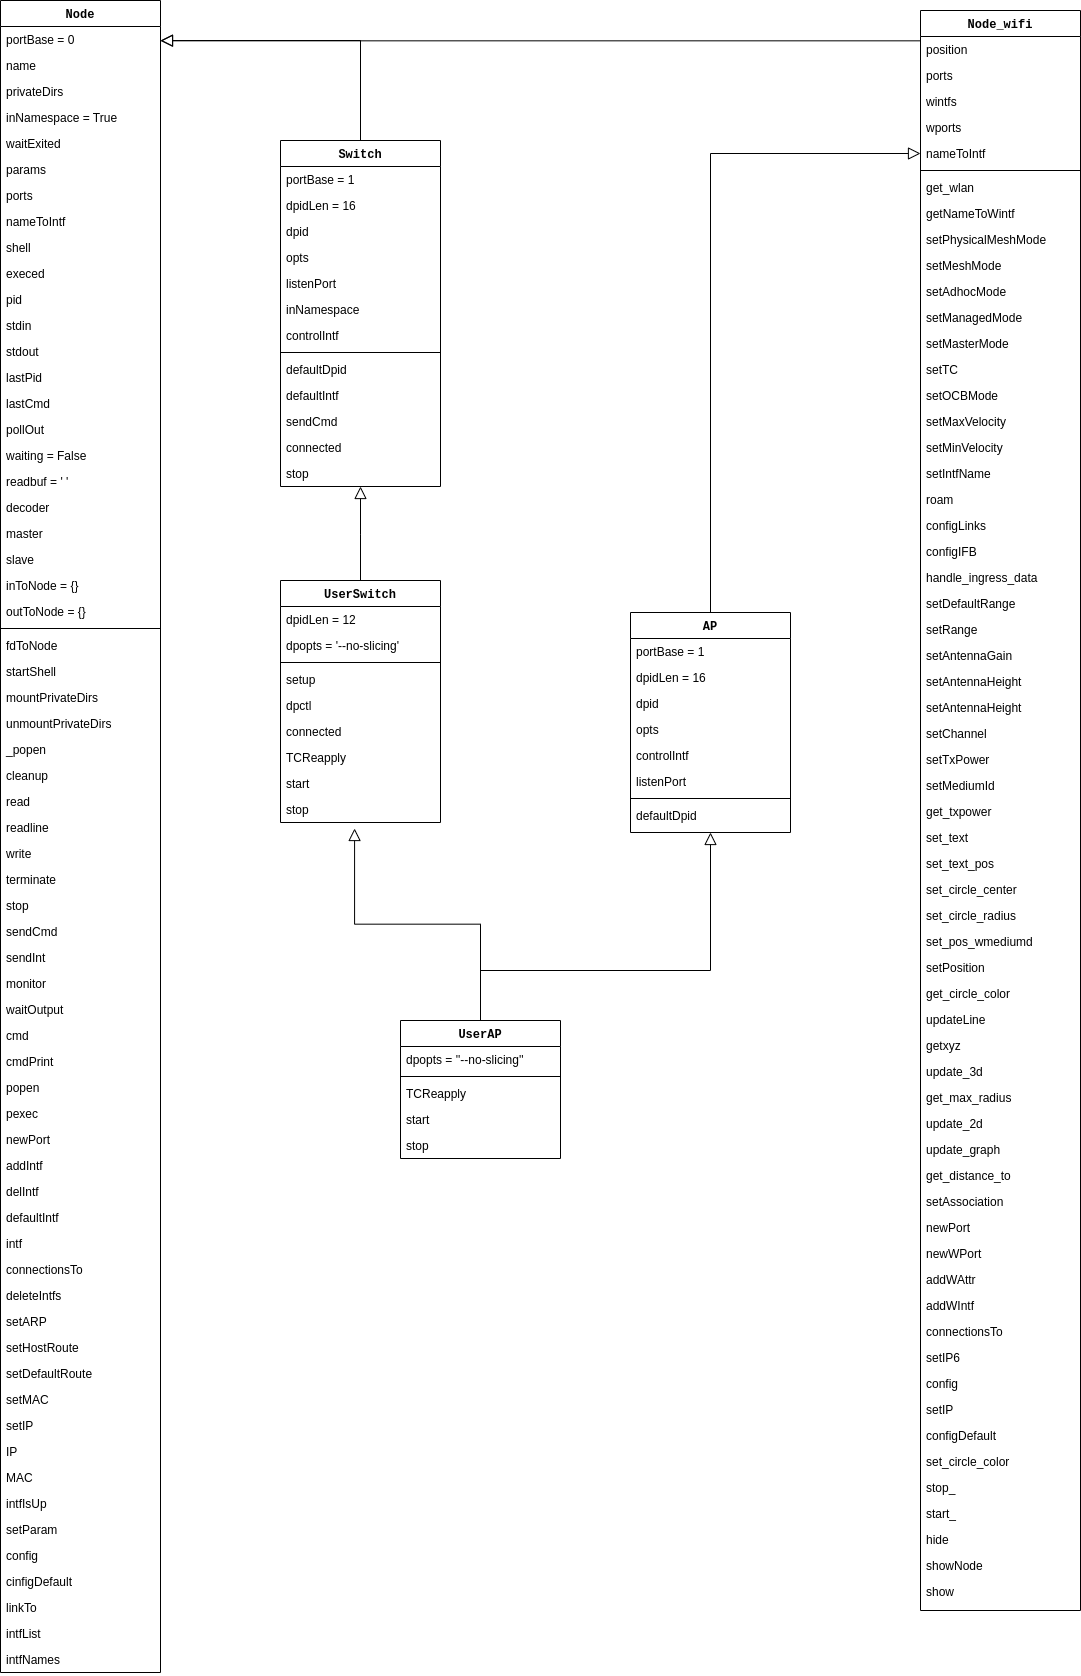
\includegraphics[width=0.8\textwidth]{archivos/img/analisis/userAP.png}
    \caption{Diagrama UML de la clase \texttt{UserAP} \cite{carrascal2023comprehensive}}
    \label{fig:userAP}
\end{figure}

%%%%%%%%%%%%%%%%%%%%%%%%%%%%%%%%%%%%%%%%%%%%%%%%%%%%%%%%%%%%%%%%%%%%%%%%%%%%%%%%%%%%%%%%%%%%%%%%%
\section{Análisis del entorno de depuración del \glsentryshort{bofus}}
\label{sec:ana_gdb}


%%%%%%%%%%%%%%%%%%%%%%%%%%%%%%%%%%%%%%%%%%%%%%%%%%%%%%%%%%%%%%%%%%%%%%%%%%%%%%%%%%%%%%%%%%%%%%%%%
